A brief description of the general design context, the general approach and the overall design of the system with its processes is presented in this section of the DD.
Our system will be developed as a 4-tiered JEE application, divided as Client Tier, Web Tier, Business Tier and the EIS Tier. It is distributed between client machines, Java EE server machine and the database.
\\The mobile and web applications in particular are thin since data operations will be computed by a central server; in this way there is no heavy load on user side clients. We think that this is the most feasible approach because the two applications have the same goals. 
\\The diagram below provides a better understanding of the components of our system, highlighting the interactions among them:
%\subsubsection{Architecture Component Diagram}
\begin{figure}[!ht]
  \centering
  \vspace{0.2cm}
  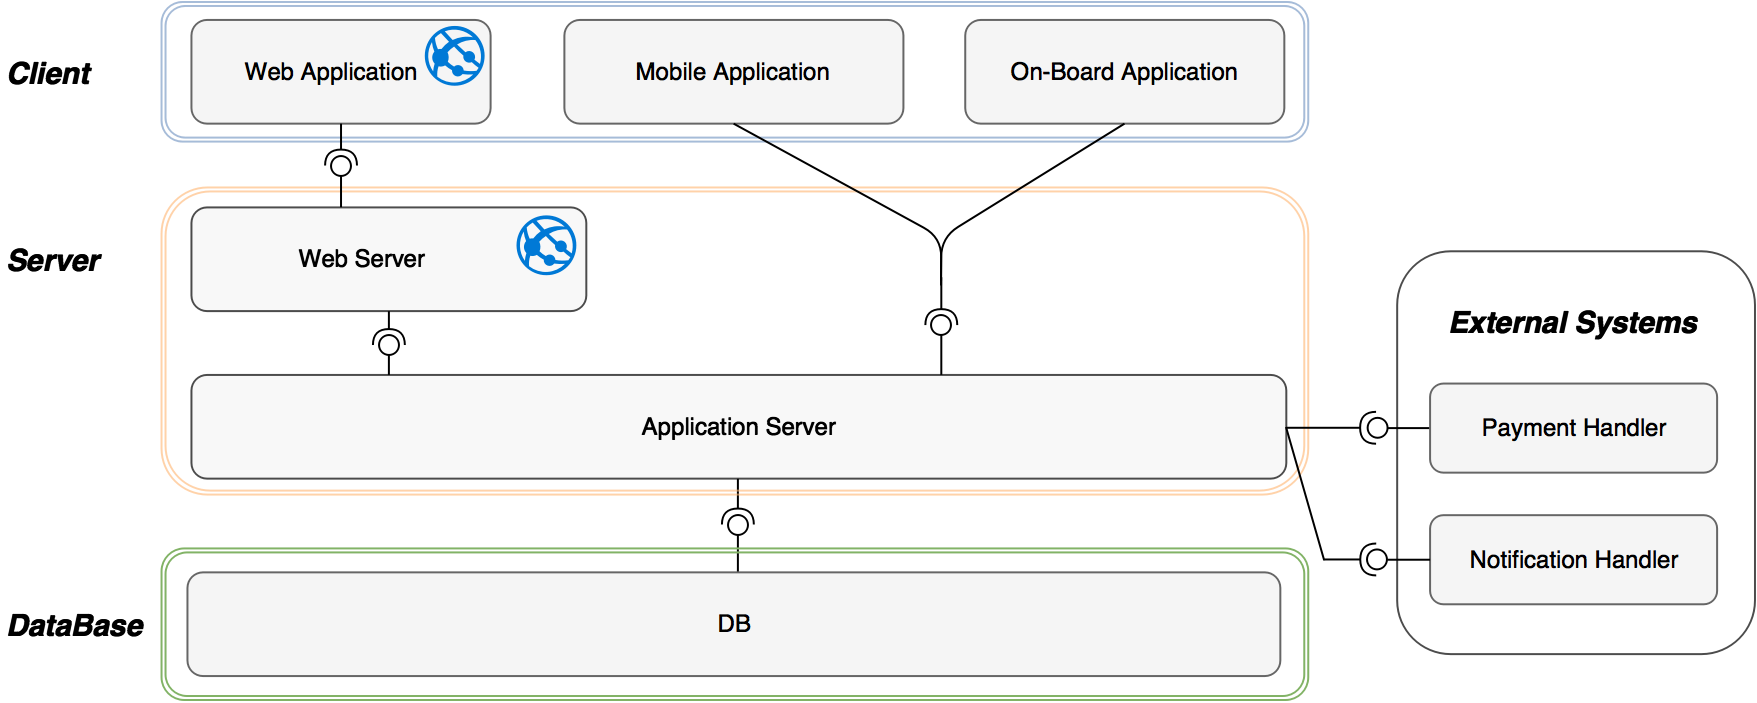
\includegraphics[width=1.0\textwidth]{/DD/architecture}\\
  \vspace{0.4cm}
  \caption{Components Diagram} 
  \label{fig:4-Tier_Architecture} 
\end{figure}

This represent a high level view of the design of the system, were is highlighted the distribution of the system over the three locations and the interaction between the different tiers thanks to their interfaces.
\\The Client Tier is composed by the On-board computer, the mobile application and the web application.
\\The Web Tier and the Business Tier are inside the server machine. We can observe that the Web application need to interact with the Web Server before to access to the Application server while the mobile application has a direct access to it.
\\The EIS Tier consists in a database that store all the system's data and interact through the DB Interface with the server.
